\documentclass[a4paper]{book}
\usepackage{makeidx}
\usepackage{graphicx}
\usepackage{multicol}
\usepackage{float}
\usepackage{listings}
\usepackage{color}
\usepackage{ifthen}
\usepackage[table]{xcolor}
\usepackage{textcomp}
\usepackage{alltt}
\usepackage{ifpdf}
\ifpdf
\usepackage[pdftex,
            pagebackref=true,
            colorlinks=true,
            linkcolor=blue,
            unicode
           ]{hyperref}
\else
\usepackage[ps2pdf,
            pagebackref=true,
            colorlinks=true,
            linkcolor=blue,
            unicode
           ]{hyperref}
\usepackage{pspicture}
\fi
\usepackage[utf8]{inputenc}
\usepackage[french]{babel}

\usepackage{mathptmx}
\usepackage[scaled=.90]{helvet}
\usepackage{courier}
\usepackage{sectsty}
\usepackage[titles]{tocloft}
\usepackage{doxygen}
\lstset{language=C++,inputencoding=utf8,basicstyle=\footnotesize,breaklines=true,breakatwhitespace=true,tabsize=8,numbers=left }
\makeindex
\setcounter{tocdepth}{3}
\renewcommand{\footrulewidth}{0.4pt}
\renewcommand{\familydefault}{\sfdefault}
\begin{document}
\hypersetup{pageanchor=false}
\begin{titlepage}
\vspace*{7cm}
\begin{center}
{\Large Dr.Robotnik Mean Bean Machine \\[1ex]\large 1.0 }\\
\vspace*{1cm}
{\large Généré par Doxygen 1.7.4}\\
\vspace*{0.5cm}
{\small Mon May 9 2011 00:31:57}\\
\end{center}
\end{titlepage}
\clearemptydoublepage
\pagenumbering{roman}
\tableofcontents
\clearemptydoublepage
\pagenumbering{arabic}
\hypersetup{pageanchor=true}
\chapter{Index des fichiers}
\section{Liste des fichiers}
Liste de tous les fichiers avec une brève description :\begin{DoxyCompactList}
\item\contentsline{section}{\hyperlink{a00001}{main.cpp} }{\pageref{a00001}}{}
\item\contentsline{section}{source/\hyperlink{a00002}{DashBoard.cpp} }{\pageref{a00002}}{}
\item\contentsline{section}{source/\hyperlink{a00003}{Game.cpp} }{\pageref{a00003}}{}
\item\contentsline{section}{source/\hyperlink{a00004}{Grille.cpp} }{\pageref{a00004}}{}
\item\contentsline{section}{source/\hyperlink{a00005}{InterfaceX.cpp} }{\pageref{a00005}}{}
\item\contentsline{section}{source/\hyperlink{a00006}{MoteurPhy.cpp} }{\pageref{a00006}}{}
\end{DoxyCompactList}

\chapter{Documentation des fichiers}
\hypertarget{a00001}{
\section{Référence du fichier main.cpp}
\label{a00001}\index{main.cpp@{main.cpp}}
}
{\ttfamily \#include \char`\"{}include/Game.h\char`\"{}}\par
Graphe des dépendances par inclusion de main.cpp:
\nopagebreak
\begin{figure}[H]
\begin{center}
\leavevmode
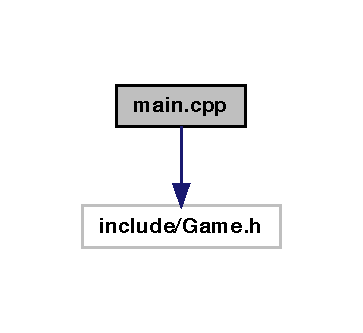
\includegraphics[width=174pt]{a00008}
\end{center}
\end{figure}
\subsection*{Fonctions}
\begin{DoxyCompactItemize}
\item 
int \hyperlink{a00001_a0ddf1224851353fc92bfbff6f499fa97}{main} (int argc, char $\ast$argv\mbox{[}$\,$\mbox{]})
\begin{DoxyCompactList}\small\item\em Fonction de cr�ation d'une nouvelle instance d'un objet Str\_\-t. \end{DoxyCompactList}\end{DoxyCompactItemize}


\subsection{Documentation des fonctions}
\hypertarget{a00001_a0ddf1224851353fc92bfbff6f499fa97}{
\index{main.cpp@{main.cpp}!main@{main}}
\index{main@{main}!main.cpp@{main.cpp}}
\subsubsection[{main}]{\setlength{\rightskip}{0pt plus 5cm}int main (
\begin{DoxyParamCaption}
\item[{int}]{argc, }
\item[{char $\ast$}]{argv\mbox{[}$\,$\mbox{]}}
\end{DoxyParamCaption}
)}}
\label{a00001_a0ddf1224851353fc92bfbff6f499fa97}


Fonction de cr�ation d'une nouvelle instance d'un objet Str\_\-t. 


\begin{DoxyParams}{Paramètres}
{\em argc} & essai argv essai2 \\
\hline
\end{DoxyParams}
\begin{DoxyReturn}{Renvoie}
zero. 
\end{DoxyReturn}


Définition à la ligne 9 du fichier main.cpp.


\hypertarget{a00002}{
\section{Référence du fichier source/DashBoard.cpp}
\label{a00002}\index{source/DashBoard.cpp@{source/DashBoard.cpp}}
}
{\ttfamily \#include \char`\"{}../include/DashBoard.h\char`\"{}}\par
Graphe des dépendances par inclusion de DashBoard.cpp:
\nopagebreak
\begin{figure}[H]
\begin{center}
\leavevmode
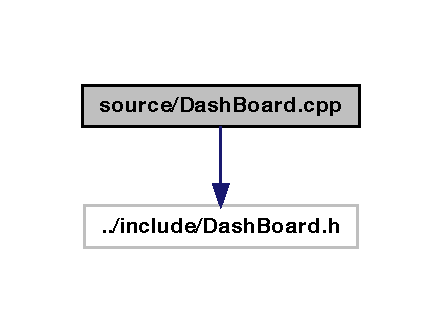
\includegraphics[width=212pt]{a00009}
\end{center}
\end{figure}

\hypertarget{a00003}{
\section{Référence du fichier source/Game.cpp}
\label{a00003}\index{source/Game.cpp@{source/Game.cpp}}
}
{\ttfamily \#include \char`\"{}../include/Game.h\char`\"{}}\par
{\ttfamily \#include \char`\"{}../include/InterfaceX.h\char`\"{}}\par
Graphe des dépendances par inclusion de Game.cpp:
\nopagebreak
\begin{figure}[H]
\begin{center}
\leavevmode
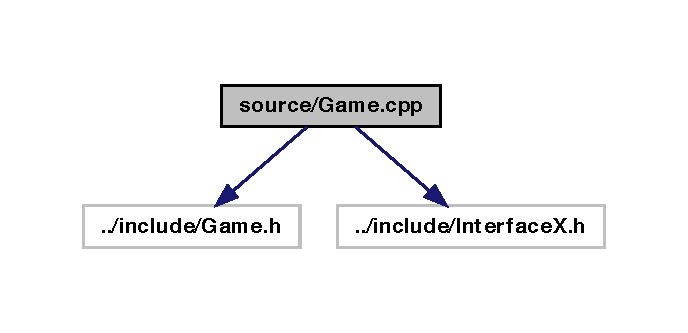
\includegraphics[width=330pt]{a00010}
\end{center}
\end{figure}

\hypertarget{a00004}{
\section{Référence du fichier source/Grille.cpp}
\label{a00004}\index{source/Grille.cpp@{source/Grille.cpp}}
}
{\ttfamily \#include \char`\"{}../include/Grille.h\char`\"{}}\par
Graphe des dépendances par inclusion de Grille.cpp:
\nopagebreak
\begin{figure}[H]
\begin{center}
\leavevmode
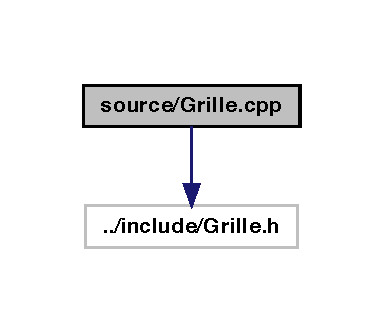
\includegraphics[width=184pt]{a00011}
\end{center}
\end{figure}

\hypertarget{a00005}{
\section{Référence du fichier source/InterfaceX.cpp}
\label{a00005}\index{source/InterfaceX.cpp@{source/InterfaceX.cpp}}
}
{\ttfamily \#include \char`\"{}../include/InterfaceX.h\char`\"{}}\par
Graphe des dépendances par inclusion de InterfaceX.cpp:
\nopagebreak
\begin{figure}[H]
\begin{center}
\leavevmode
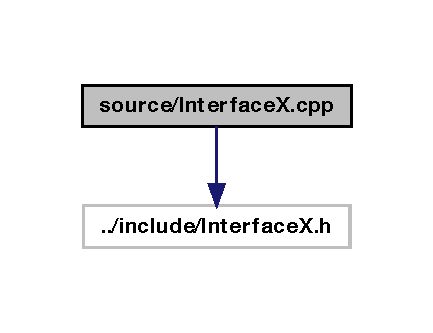
\includegraphics[width=208pt]{a00012}
\end{center}
\end{figure}

\hypertarget{a00006}{
\section{Référence du fichier source/MoteurPhy.cpp}
\label{a00006}\index{source/MoteurPhy.cpp@{source/MoteurPhy.cpp}}
}
{\ttfamily \#include \char`\"{}../include/MoteurPhy.h\char`\"{}}\par
Graphe des dépendances par inclusion de MoteurPhy.cpp:
\nopagebreak
\begin{figure}[H]
\begin{center}
\leavevmode
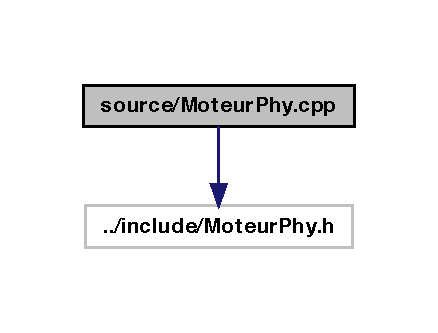
\includegraphics[width=210pt]{a00013}
\end{center}
\end{figure}

\printindex
\end{document}
